\subsection{Problem 2.1:}
Cho tín hiệu rời rạc:
\[
x(n) = \begin{cases}
1 + \frac{n}{3}, & -3 \le n \le -1 \\
1, & 0 \le n \le 3 \\
0, & \text{khác}
\end{cases}
\]

\begin{enumerate}
    \item Xác định các giá trị và vẽ tín hiệu $x(n)$:\\
    Thay các giá trị $n \in [-3, 3]$ vào $x(n)$, ta có:
    \[
    \begin{cases}
        x(-3) = 1 + \frac{-3}{3} = 0 \\
        x(-2) = 1 + \frac{-2}{3} = \frac{1}{3} \\
        x(-1) = 1 + \frac{-1}{3} = \frac{2}{3} \\
        x(0) = x(1) = x(2) = x(3) = 1 \\
        x(n) = 0 \text{ khi } n \text{ khác}
    \end{cases}
    \]
    $\rightarrow$ Dãy tín hiệu thu được: $x(n) = \{0, \frac{1}{3}, \frac{2}{3}, \underset{\uparrow}{1}, 1, 1, 1\}$ với gốc tại $n = 0$.

    \item Vẽ các tín hiệu:
    \begin{enumerate}
        \item Fold $x(n)$ trước rồi delay tín hiệu kết quả 4 mẫu:
        \begin{itemize}
            \item Fold: $v(n) = x(-n)$
            \item Delay 4 mẫu: $x_1(n) = v(n - 4) = x(-(n - 4)) = x(-n + 4)$
        \end{itemize}
        $\rightarrow$ Tín hiệu tồn tại trong khoảng $-3 \le -n + 4 \le 3 \leftrightarrow 1 \le n \le 7$.\\
        $\rightarrow$ Dãy tín hiệu: $x_1(n) = \{0, \underset{\uparrow}{0}, 1, 1, 1, 1, \frac{2}{3}, \frac{1}{3}, 0\}$ ($n \in [0, 7]$).

        \item Delay $x(n)$ 4 mẫu trước rồi fold tín hiệu kết quả:
        \begin{itemize}
            \item Delay 4 mẫu: $w(n) = x(n - 4)$
            \item Fold: $x_2(n) = w(-n) = x(-n - 4)$
        \end{itemize}
        $\rightarrow$ Tín hiệu tồn tại trong khoảng $-3 \le -n - 4 \le 3 \leftrightarrow -7 \le n \le -1$.\\
        $\rightarrow$ Dãy tín hiệu: $x_2(n) = \{0, \frac{1}{3}, \frac{2}{3}, 1, 1, 1, 1, \underset{\uparrow}{0}\}$ ($n \in [-7, 0]$).
    \end{enumerate}

    \item Vẽ tín hiệu $x(-n + 4)$:\\
    Ta có: $x(-n + 4)$ chính là tín hiệu $x_1(n)$ ở câu 2a (Fold trước rồi Delay 4 mẫu).\\
    Tín hiệu nhận các giá trị khác 0 tại $n \in [1, 6]$:
    \[
    x(-n + 4) = \begin{cases}
    1, & n = 1, 2, 3, 4 \\
    \frac{2}{3}, & n = 5 \\
    \frac{1}{3}, & n = 6 \\
    0, & \text{khác}
    \end{cases}
    \]

    \item So sánh kết quả câu 2 và 3, rút ra quy tắc tổng quát để có $x(-n + k)$ từ $x(n)$:\\
    \textbf{So sánh:}\\
    Kết quả tín hiệu $x(-n + 4)$ ở câu 3 giống hoàn toàn với câu 2a (Fold trước rồi Delay 4 mẫu), và khác với câu 2b (Delay 4 mẫu rồi Fold ra $x(-n - 4)$).\\
    \textbf{Quy tắc tổng quát để tạo tín hiệu $x(-n + k)$ từ $x(n)$:}
    \begin{itemize}
        \item Cách 1 (Fold trước rồi Shift):
        $$
        x(n) \xrightarrow{\text{Fold}} x(-n) \xrightarrow{\text{Delay } k \text{ mẫu: } n \to n - k} x(-(n - k)) = x(-n + k)
        $$
        \item Cách 2 (Shift trước rồi Fold):
        $$
        x(n) \xrightarrow{\text{Advance } k \text{ mẫu: } n \to n + k} x(n + k) \xrightarrow{\text{Fold: } n \to -n} x(-n + k)
        $$
    \end{itemize}
    \textbf{Kết luận:} Phép đảo (fold) và phép dịch (shift) không có tính giao hoán. Nếu dịch trước rồi đảo thì phải dịch sớm $k$ mẫu, còn nếu đảo trước rồi dịch thì phải dịch trễ $k$ mẫu.

    \item Biểu diễn $x(n)$ theo $\delta(n)$ và $u(n)$:\\
    - Theo $\delta(n)$:
    \[
    x(n) = \frac{1}{3}\delta(n + 2) + \frac{2}{3}\delta(n + 1) + \delta(n) + \delta(n - 1) + \delta(n - 2) + \delta(n - 3)
    \]
    - Theo $u(n)$:
    \[
    x(n) = \frac{1}{3}u(n + 2) + \frac{1}{3}u(n + 1) + \frac{1}{3}u(n) - u(n - 4)
    \]
\end{enumerate}

\begin{figure}[H]
    \centering
    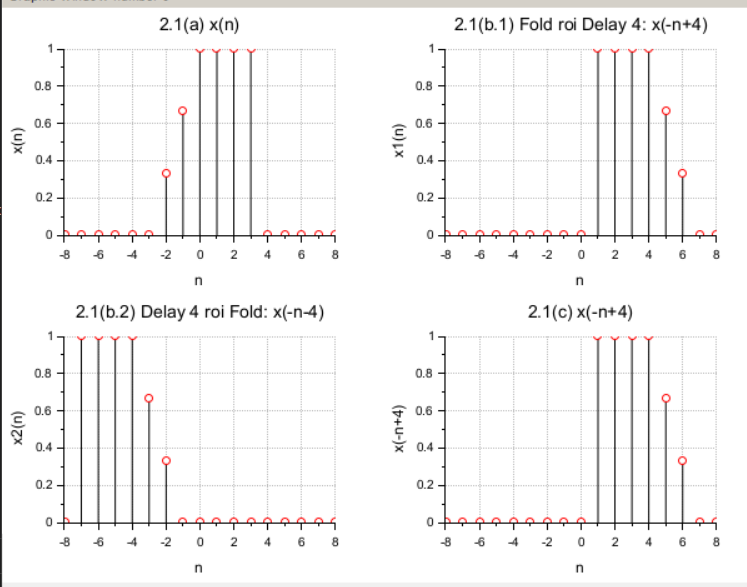
\includegraphics[width=0.75\textwidth]{img/ad_ex2.1.png}
    \caption{Đồ thị mô phỏng kết quả Problem 2.1 trên Scilab}
\end{figure}
